\chapter{Configuration space}

A robot from a mechanical point of view can be seen as a system of $N$ rigid bodies that move in a workspace $W = \mathbb{R} ^2$ or $W = \mathbb{R} ^3$.
The workspace $W$ is the physical space in which the robot operates and can move, it's essentially the geometric space in which the robot operates and can move.
If the workspace is $\mathbb{R} ^2$, the robot is called planar, if the workspace is $\mathbb{R} ^2$ the robot is called spatial.
This definition of a robot is broad enough to allow a group of robots to be defined as a robot.

\begin{definition}
    A configuration $\bm{q}$ is the minimal set of values that fully describe the position and orientation (pose) of the robot (of every point of the robot) at a given time in the workspace.
    $$
        \bm{q} = \begin{bmatrix}
            q_1    \\
            \vdots \\
            q_n
        \end{bmatrix}
    $$
\end{definition}




The components $q_i, \ i =1\dots n$ of a configuration are called generalized components.
The name generalized comes from the fact that the coordinates aren't limited to express only rotations or translations, in fact they can represent any type of motion.
These coordinates generalize the description of the robot’s motion, meaning they adapt to any kind of mechanical system, whether it’s a simple 1D slider or a complex multi-jointed arm in 3D space.

\begin{warningbox}[Warning]
    The special orthonormal group $SO(3)$ describes the orientation of a body using a $3 \times 3$ rotation matrix. Although straightforward, this method is not minimal, as the matrix has 9 elements, with only 3 being independent due to orthonormality constraints, leading to redundancy.

    Euler angles offer a minimal alternative by using 3 parameters (roll, pitch, yaw) to represent the 3 degrees of freedom. However, they suffer from gimbal lock, a singularity where two rotational axes align, causing the loss of one degree of freedom.

    Quaternions, a four-dimensional extension of complex numbers, avoid gimbal lock and efficiently represent rotations. However, they are not minimal either, requiring 4 parameters and a normalization constraint, which introduces redundancy.

    While quaternions are more robust, Euler angles may still be preferred for their minimality, despite the risk of gimbal lock, due to their simpler and more compact representation.
\end{warningbox}

\begin{definition}
    A configuration space $\mathbf{C}$ as the set containing all valid configurations.

    $$
        \mathbf{C}  \{\bm{q} \in \mathbb{R} | \bm{q} \ \text{is a valid configuration of the robot}\}
    $$
\end{definition}

\begin{example}
    Assume we have a robot with a negligible dimension w.r.t to to the workspace $W = \mathbb{R}^3$
    \begin{center}
        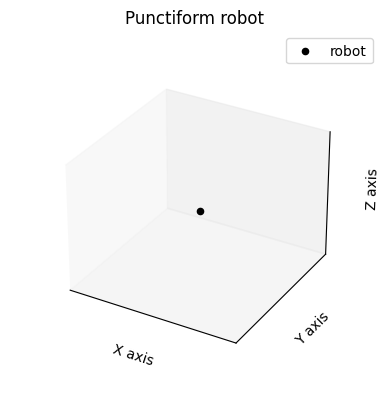
\includegraphics{Configuration space/punctiform_robot.png}
    \end{center}


    In this case the configuration vector is the following
    $$
        \bm{q} = \begin{bmatrix}
            x \\
            y \\
            z
        \end{bmatrix}
    $$
    \begin{tipbox}[Tip]
        In this case $\mathbf{C} = W = \mathbb{R}^3$, this however is not true in general.
    \end{tipbox}
\end{example}

\begin{example}
    Assume we have a circular symmetric robot in the plane, i.e. workspace $W = \mathbb{R}^2$.
    \begin{center}
        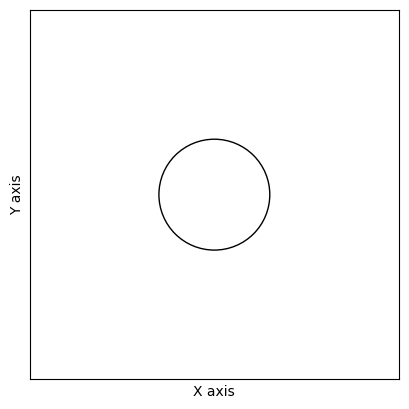
\includegraphics{Configuration space/symmetric_roomba.png}
    \end{center}

    By exploiting it's symmetry, we can express the position of all of it's points w.r.t the center of mass of the robot
    $$
        \bm{q} = \begin{bmatrix}
            x \\
            y
        \end{bmatrix}
    $$
\end{example}

\begin{example}
    Assume we have a circular symmetric robot in the plane, i.e. workspace $W = \mathbb{R}^2$. Now assume that it has a tick on it.

    Now assume this two configurations:

    \begin{center}
        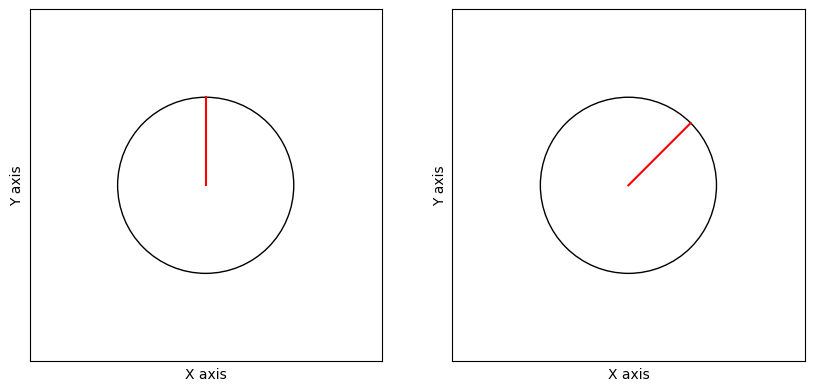
\includegraphics[width=15cm]{Configuration space/asymmetric_roomba.png}
    \end{center}

    If we where to use the previous configuration space we could not distinguish between this two configurations, because while previosly we didn't need to add rotational information, now it's required, thus the generalized vector is:

    $$
        \bm{q} = \begin{bmatrix}
            x \\
            y \\
            \theta
        \end{bmatrix}
    $$

    In which $\theta$ is for example a rotation around the $x$-axis.

    \begin{tipbox}[Tip]
        In this case $\mathbf{C} = \mathbb{R}^2 \times SO(2)$.
    \end{tipbox}

    \begin{warningbox}[Warning]
        While the $SO(3)$ group is redundant, the $SO(3)$  is not, which means that $SO(2)$ is minimal and correctly used.
    \end{warningbox}

    Now, we can represent, for example a positive movement along the $x$ axis as

    \begin{center}
        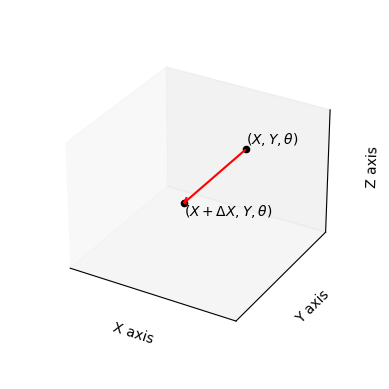
\includegraphics{Configuration space/naive_asymmetric_roomba_configuration_space.png}
    \end{center}

    This is actually \textbf{not} a good representation of the configuration space, however it is convenient because it let's us compress our robot from a volume into a point.
    The need of the configuration space is infact given by the abstraction of the robots geometry.
\end{example}

\begin{example}
    Assume you have a planar manipulator with $N$ joints.

    \begin{center}
        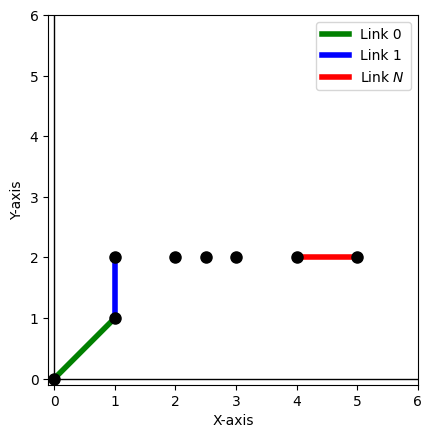
\includegraphics{Configuration space/multi_joint.png}
    \end{center}

    We could describe the configuration of this manupulator by taking as a position the baricenter of each link and thei inclination of each joint, this results in $3N$ parameters.
    This configuration would be great, however it is not minimal.
    A problem, is that assumes that there is no relationship between the links, however we know that the joint pose a constraint which make them dependant.
    Since each joint introduces 2 constraints, the number of free parameters is $3N-2N = N$.

    We can describe the $N$ parameters as

    \begin{center}
        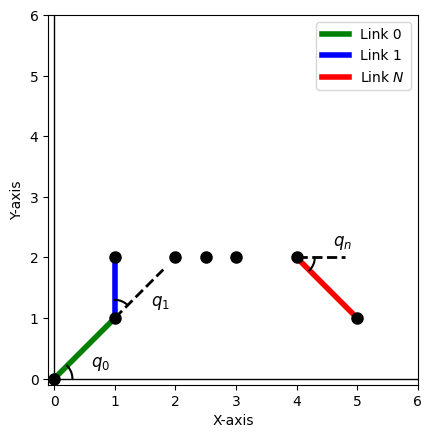
\includegraphics{Configuration space/multi_join_configuration.png}
    \end{center}

    And thus our configuration $\bm{q}$, is just:

    $$
        \bm{q} = \begin{pmatrix}
            q_0    \\
            \vdots \\
            q_n
        \end{pmatrix}
    $$

    While the configuration space is $\mathbf{C} = SO(2)^N$.

    Now, if we assume we have a spatial manipulator, we have $6N$ parameters, of which $3N$ describe the position and $3N$ describe the rotation.
    For everything we said until now, this representation is not minimal, and due to the presence of joints there are $5N$ constraints, which means that we can treat the spatial manipulator as a planar manipulator.
\end{example}